
\documentclass{beamer}
\usecolortheme{dove}
\setbeamertemplate{navigation symbols}{}
\usepackage{amsmath,amssymb,amsfonts,amsthm, multicol, subfigure, color}
\usepackage{bm}
\usepackage{graphicx}
\usepackage{tabularx}
\usepackage{booktabs}
\usepackage{hyperref}
\usepackage{pdfpages}
\usepackage{xcolor}
\definecolor{seagreen}{RGB}{46, 139, 87}
\def\independenT#1#2{\mathrel{\rlap{$#1#2$}\mkern2mu{#1#2}}}
\newcommand\indep{\protect\mathpalette{\protect\independenT}{\perp}}
\def\log{\text{log}}
\newcommand\logit{\text{logit}}
\newcommand\iid{\stackrel{\text{iid}}{\sim}}
\newcommand\E{\text{E}}
\newcommand\V{\text{V}}
\renewcommand\P{\text{P}}
\newcommand{\Cov}{\text{Cov}}
\newcommand{\Cor}{\text{Cor}}
\newcommand\doop{\texttt{do}}
\usepackage{stackrel}
\usepackage{tikz}
\usetikzlibrary{arrows,shapes.arrows,positioning,shapes,patterns,calc}
\newcommand\slideref[1]{\vskip .1cm \tiny \textcolor{gray}{{#1}}}
\newcommand\red[1]{\color{red}#1}
\newcommand\blue[1]{\color{blue}#1}
\newcommand\gray[1]{\color{gray}#1}
\newcommand\seagreen[1]{\color{seagreen}#1}
\newcommand\purple[1]{\color{purple}#1}
\newcommand\orange[1]{\color{orange}#1}
\newcommand\black[1]{\color{black}#1}
\newcommand\white[1]{\color{white}#1}
\newcommand\teal[1]{\color{teal}#1}
\newcommand\magenta[1]{\color{magenta}#1}
\newcommand\Fuchsia[1]{\color{Fuchsia}#1}
\newcommand\BlueGreen[1]{\color{BlueGreen}#1}
\newcommand\bblue[1]{\textcolor{blue}{\textbf{#1}}}
\newcommand\bred[1]{\textcolor{red}{\textbf{#1}}}
\newcommand\bgray[1]{\textcolor{gray}{\textbf{#1}}}
\newcommand\bgreen[1]{\textcolor{seagreen}{\textbf{#1}}}
\newcommand\bref[2]{\href{#1}{\color{blue}{#2}}}
\colorlet{lightgray}{gray!40}
\pgfdeclarelayer{bg}    % declare background layer for tikz
\pgfsetlayers{bg,main} % order layers for tikz
\newcommand\mycite[1]{\begin{scriptsize}\textcolor{darkgray}{(#1)}\end{scriptsize}}
\newcommand{\tcframe}{\frame{
%\small{
\only<1|handout:0>{\tableofcontents}
\only<2|handout:1>{\tableofcontents[currentsubsection]}}
%}
}

\newcommand{\goalsframe}{\begin{frame}{Learning goals for today}
By the end of class, you will be able to
\begin{itemize}
    \item understand the notion of supervised machine learning
    \begin{itemize}
    \item an input-output machine
    \item learned on some learning cases
    \item used to predict for new cases
    \end{itemize}
    \item apply that notion to the specific case of regression trees
    \item read a prediction from a regression tree
    \item understand how trees can aggregate to a forest
 \end{itemize} 
  \vskip .2in
\end{frame}}

\usepackage[round]{natbib}
\bibliographystyle{humannat-mod}
\setbeamertemplate{enumerate items}[default]
\usepackage{mathtools}

\title{Studying Social Inequality with Data Science}
\author{Ian Lundberg}
\date{\today}

\begin{document}

\begin{frame}
\begin{tikzpicture}[x = \textwidth, y = \textheight]
\node at (0,0) {};
\node at (1,1) {};
\node[anchor = north west, align = left, font = \huge] at (0,.9) {Social\\Data\\Science};
\node[anchor = north east, align = right] (number) at (1,.9) {Soc 114\\Winter 2026};
\node[anchor = north, font = \Large, align = center] at (.5,.5) {Supervised Machine Learning:\\Trees and Forests};
\end{tikzpicture}
\end{frame}

\goalsframe

\begin{frame}{Prediction function and supervised learning}

A \textbf{prediction function} is an input-output function:
\begin{itemize}
\item input a vector of predictors $\vec{x}$
\item output a predicted outcome $\hat{y} = \hat{f}(\vec{x})$
\end{itemize}

\begin{center}
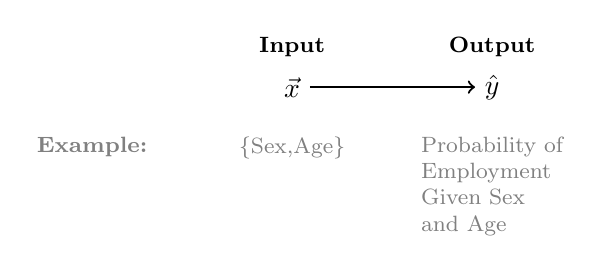
\begin{tikzpicture}[x = 1in, y = .2in]
\node (x) at (1,0) {$\vec{x}$};
\node (y) at (2,0) {$\hat{y}$};
\draw[->, thick] (x) -- (y);
\node[anchor = north, font = {\footnotesize\bf}] at (1,1.5) {Input};
\node[anchor = north, font = {\footnotesize\bf}] at (2,1.5) {Output};
\node[anchor = north, font = {\footnotesize\bf}, gray] at (0,-1) {Example:};
\node[anchor = north, font = \footnotesize, gray] at (1,-1) {\{Sex,Age\}};
\node[anchor = north, font = \footnotesize, gray, align = left] at (2,-1) {Probability of\\Employment\\Given Sex\\and Age};
\end{tikzpicture}
\end{center}
\textbf{Supervised learning} includes any approach that uses observed $\{\vec{x},y\}$ data to learn a prediction function $\hat{f}$

\end{frame}

\begin{frame}
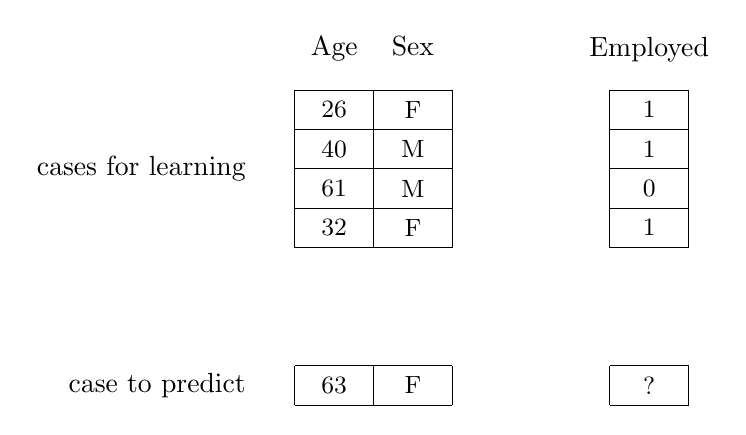
\begin{tikzpicture}
\node[anchor = north] at (.5,2.8) {Age};
\node[anchor = north] at (1.5,2.8) {Sex};
\node[anchor = north] at (4.5,2.8) {Employed};
% Learning grids
\draw[xstep = 1, ystep = .5] (0,0) grid (2,2);
\draw[xstep = 1, ystep = .5] (4,0) grid (5,2);
% Prediction grid
\draw[xstep = 1, ystep = .5] (0,-2) grid (2,-1.5);
\draw[xstep = 1, ystep = .5] (4,-2) grid (5,-1.5);
% Ages
\node[font = \small] at (.5,1.75) {26};
\node[font = \small] at (.5,1.25) {40};
\node[font = \small] at (.5,.75) {61};
\node[font = \small] at (.5,.25) {32};
% Sexes
\node[font = \small] at (1.5,1.75) {F};
\node[font = \small] at (1.5,1.25) {M};
\node[font = \small] at (1.5,.75) {M};
\node[font = \small] at (1.5,.25) {F};
% Employment
\node[font = \small] at (4.5,1.75) {1};
\node[font = \small] at (4.5,1.25) {1};
\node[font = \small] at (4.5,.75) {0};
\node[font = \small] at (4.5,.25) {1};
% To predict
\node[font = \small] at (.5,-1.75) {63};
\node[font = \small] at (1.5,-1.75) {F};
\node[font = \small] at (4.5,-1.75) {?};
% Label cases
\node[anchor = east, align = right] at (-.5,1) {cases for learning};
\node[anchor = east, align = right] at (-.5,-1.75) {case to predict};
\end{tikzpicture}
\end{frame}

\begin{frame}{OLS is a prediction function}{$\text{Input }\vec{x}\rightarrow \text{Output }\hat{y}$}

$$
\hat{y} = \hat{f}(\vec{x}) = \hat\beta_0 + \hat\beta_1(\text{Sex = Male}) + \hat\beta_2(\text{Age})
$$
\begin{itemize}
\item Learn $\hat{f}$ in a \textbf{learning sample} with $\{\vec{x}_i,y_i\}_{i=1}^n$
\begin{itemize}
\item Computer finds $\hat\beta_0$, $\hat\beta_1$, $\hat\beta_2$ that predict well in the learning sample
\end{itemize}
\item At a new $\vec{x}$ value, predict $\hat{f}(\vec{x})$
\end{itemize}

\end{frame}

\begin{frame}{Logistic regression is a prediction function}{$\text{Input }\vec{x}\rightarrow \text{Output }\hat{y}$}

$$
\hat{y} = \hat{f}(\vec{x}) = \text{logit}^{-1}\left(\hat\beta_0 + \hat\beta_1(\text{Sex = Male}) + \hat\beta_2(\text{Age})\right)
$$
\begin{itemize}
\item Learn $\hat{f}$ in a \textbf{learning sample} with $\{\vec{x}_i,y_i\}_{i=1}^n$
\begin{itemize}
\item Computer finds $\hat\beta_0$, $\hat\beta_1$, $\hat\beta_2$ that predict well in the learning sample
\end{itemize}
\item At a new $\vec{x}$ value, predict $\hat{f}(\vec{x})$
\end{itemize}

\end{frame}

\begin{frame}{There are many prediction functions}

\begin{itemize}
\item input a vector of predictors $\vec{x}$
\item output a predicted outcome $\hat{y} = \hat{f}(\vec{x})$
\end{itemize}

\end{frame}

\begin{frame}{Trees as a prediction function}

Tree: A series of TRUE or FALSE decisions leading to a prediction \vskip .1in
A made-up example:
\begin{itemize}
\item Is age greater than 40?
\begin{itemize}
\item If so, is the respondent labeled female?
\begin{itemize}
\item If so, predict 80\% employed
\item If not, predict 85\% employed
\end{itemize}
\item If age not greater than 40, predict 70\% employed
\end{itemize}
\end{itemize}

\end{frame}

\begin{frame}{Trees as a prediction function}

\includegraphics<1>[width = \textwidth]{figures/tree_sim_1}
\includegraphics<2>[width = \textwidth]{figures/tree_sim_2}
\includegraphics<3>[width = \textwidth]{figures/tree_sim_3}
\includegraphics<4>[width = \textwidth]{figures/tree_sim_4}
\includegraphics<5>[width = \textwidth]{figures/tree_sim_viz}

\end{frame}

\begin{frame}{Trees as a prediction function: How that worked}

\includegraphics<1>[width = \textwidth]{figures/tree_sim_1}
\includegraphics<2>[width = \textwidth]{figures/tree_choice_1}
\includegraphics<3>[width = \textwidth]{figures/tree_sim_2}
\includegraphics<4>[width = \textwidth]{figures/tree_choice_2}
\includegraphics<5>[width = \textwidth]{figures/tree_sim_3}
\includegraphics<6>[width = \textwidth]{figures/tree_sim_4}
\includegraphics<7>[width = \textwidth]{figures/tree_sim_viz}

\end{frame}

\begin{frame}{Trees as a prediction function: How that worked. \textbf{Summary.}}

\begin{enumerate}
\item Begin with all data
\item Consider many ways to partition into two parts
\item Estimate the mean squared prediction error for each: $\E((\hat{Y} - Y)^2)$
\item Choose the split that minimizes mean squared prediction error
\end{enumerate}
Repeatedly, apply steps (1--4) to each subgroup. \\
Stop by a data-driven rule.

\end{frame}

\begin{frame}{Trees: Some terminology}

\begin{itemize}
\item Branch = one direction of a split
\item Leaf = terminal node at the bottom
\end{itemize}
\begin{center}
\includegraphics[width = .7\textwidth]{figures/tree_sim_viz}
\end{center}
When presented with a new case, find its leaf.\\Predict the mean of $Y$ among learning cases in that leaf.

\end{frame}

\begin{frame}{A tree can be interpretable: Realistic example}

\begin{itemize}
\item Outcome: Has spouse or partner with BA degree at age 35
\item Predictors: Demographics and measures of family background
\end{itemize}

\end{frame}

\begin{frame}{A tree can be interpretable: Realistic example}

\includegraphics[width = \textwidth]{figures/tree_fitting_code}

\end{frame}

\begin{frame}{A tree can be interpretable: Realistic example}

$Y = $ has spouse or partner with BA degree at age 35

\includegraphics[width = \textwidth]{figures/tree_fitting_figure}

\end{frame}

\begin{frame}{Pruning a tree}
Sometimes you want a simpler decision rule
\begin{itemize}
\item you worry you are fitting to noise
\item you want to explain predictions more easily
\end{itemize} \vskip .2in \pause
Then you prune the tree: Trim back some branches

\end{frame}

\begin{frame}{Pruning a tree: Original tree}

\includegraphics[width = \textwidth]{figures/tree_fitting_figure}

\end{frame}

\begin{frame}{Pruning a tree: Pruned tree}{pruned $<$- prune(rpart.out, cp = .02)}

\includegraphics[width = \textwidth]{figures/tree_fitting_figure_pruned}

\end{frame}

\begin{frame}{Discussion: Why prefer a tree vs OLS?}

\begin{itemize}
\item Reasons to prefer a tree
\onslide<2->{
\begin{itemize}
\item No need to assume a functional form
\item Easy to explain how a prediction is made:\\follow the decision branches
\end{itemize}
}
\item Reasons to prefer OLS
\onslide<3->{
\begin{itemize}
\item More widely known in social science
\item Better if the functional form is correct
\end{itemize}
}
\end{itemize}

\end{frame}

\begin{frame}{From trees to forests}

Trees are \textbf{high-variance} estimators

\begin{itemize}
\item Suppose we all have different samples
\item We each estimate a tree
\item Trees will look very different
\end{itemize}

\end{frame}

\begin{frame}{From trees to forests}

Forests aggregate trees to \textbf{reduce variance}

\begin{itemize}
\item For tree $1,\dots,n_\text{Trees}$
\begin{itemize}
\item Bootstrap the data
\item Randomly sample $p_\text{Selected} < p$ columns of the data
\item Learn a tree
\end{itemize}
\item Then predict the average of the trees
\end{itemize}

\end{frame}

\begin{frame}{From trees to forests}

Together, we will try a forest on the course \bref{https://soc114.github.io/topics/7\_forests.html\#your-turn-a-random-forest-with-grf}{website page}

\end{frame}

\begin{frame}{From trees to forests}

Why might you prefer a tree?

Why might you prefer a forest?

\end{frame}

\goalsframe

\end{document}
